\documentclass[10pt]{article}
\usepackage[portuguese]{babel} % para indice em português
\usepackage{url}
\usepackage{graphicx}
\usepackage{float}
\graphicspath{ {./figures/} }



\begin{document}

\begin{titlepage}
	\begin{center}
		\vspace*{1cm}
		
    {\fontsize{17}{16}\selectfont \textbf{Gestão Inteligente de Inventário com Etiquetas de E-Ink e Aplicação Móvel}}
     
		
		\vspace{0.5cm}
		Relatório Final do Projeto Integrador
		
		\vspace{1.5cm}
		
		\textbf{Afonso Saraiva}\\
		\textbf{Daniel Marques}\\ %se aplicavel
		\textbf{Hugo Silva}\\ %se aplicavel
		\textbf{Inês Francisco}\\ %se aplicavel
		
				\vfill
		
		
\includegraphics[width=0.4\textwidth]{UPORTO_fundotransparente}
		
		\vfill
		
	
		
		Licenciatura em Engenharia Informática e Computação
		
		\vspace{0.8cm}
		
		
		\textbf{Tutor na U.Porto}: Eduardo Marques\\
		\textbf{Orientador na empresa/Proponente}: Filipe Sousa \\ %Se diferente do tutor

\vspace{0.4cm}
		13 de março, 2026
		
	\end{center}
\end{titlepage}


\thispagestyle{empty} 
\clearpage

\thispagestyle{empty}
\tableofcontents

 \clearpage
 
\section{Introdução}

O presente relatório descreve o trabalho desenvolvido no âmbito do projeto integrador, cujo objetivo consiste no desenvolvimento de um sistema para gestão e atualização de etiquetas eletrônicas e-ink integradas com um sistema de inventário digital.
	
	\subsection{Enquadramento}

    O projeto foi desenvolvido no contexto de um ambiente de investigação e desenvolvimento tecnológico, semelhante ao existente em organizações de investigação aplicada, como a Fraunhofer Portugal.
	
	Neste tipo de organizações, é comum existirem diversos espaços de armazenamento, como gavetas, armários ou caixas, utilizados para guardar componentes, materiais de laboratório, protótipos e equipamentos relacionados com diferentes projetos.
	
	A gestão destes materiais é frequentemente feita através de etiquetas em papel, o que origina inconsistências entre o estado real do inventário e os registos digitais existentes, dificultando a identificação rápida dos recursos disponíveis.

	\begin{figure}[H]
		\centering
		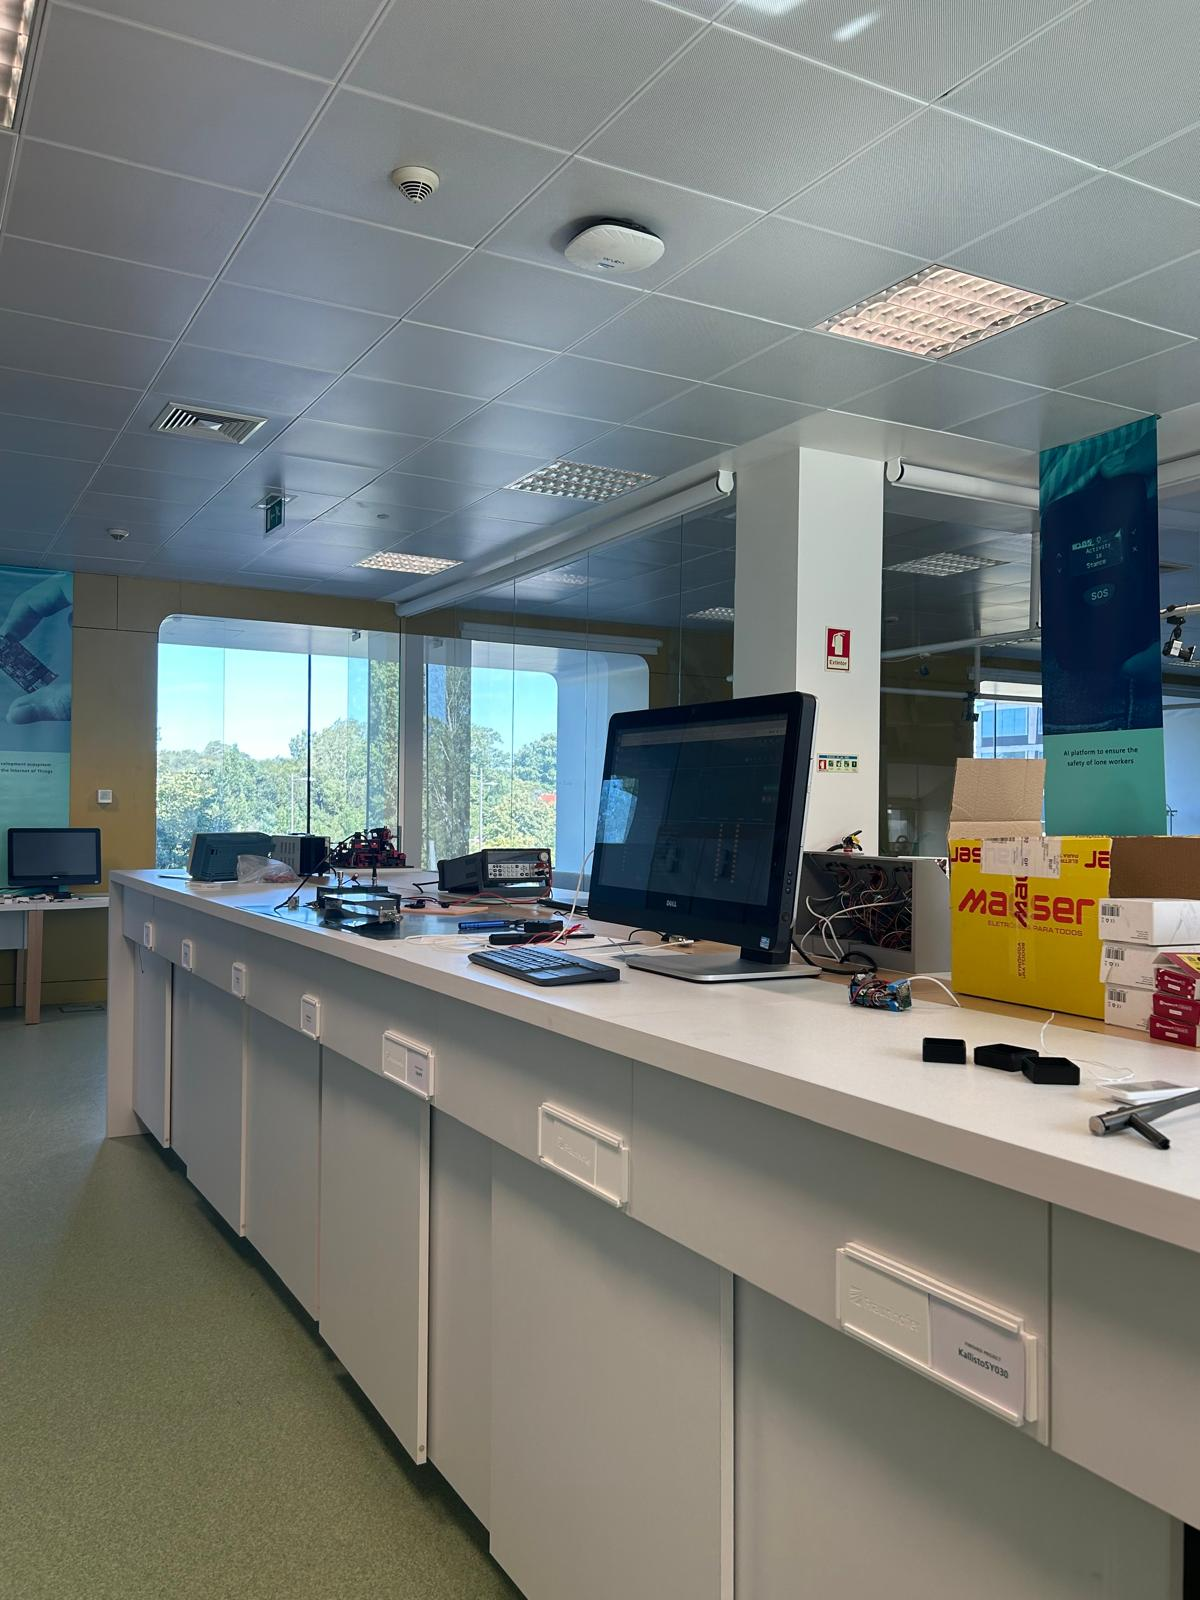
\includegraphics[width=0.6\textwidth]{FraunhoferAICOS}
		\caption{Fraunhofer Portugal AICOS}
	\end{figure}
	
	\subsection{Objetivos e resultados esperados}
	
	Reconhecendo os desafios da gestão de inventário, o projeto visou desenvolver um sistema que permitisse manter as etiquetas físicas das gavetas automaticamente sincronizadas com a informação da base de dados do inventário.

	Os objetivos principais foram integrar etiquetas e-ink com o Inventree, de forma a que qualquer alteração no nome de uma localização se reflita automaticamente na etiqueta física correspondente. Além disso, desenvolver uma aplicação móvel que permitisse ao utilizador consultar o stock e gerir o inventário através da leitura de um código QR.
	
	Desta forma, o sistema deverá eliminar a necessidade de atualização manual de etiquetas, garantindo que a informação física está sempre consistente com os registos digitais.
    
	\subsection{Estrutura do relatório}
	
	Este relatório está estruturado em quatro seções. A Seção 1 apresenta uma introdução ao projeto, incluindo o contexto, os objetivos e os resultados esperados. 
	A Seção 2 descreve a metodologia e as principais atividades realizadas durante o projeto, abrangendo a metodologia utilizada, as partes interessadas envolvidas e as atividades desenvolvidas. 
	A Seção 3 apresenta o desenvolvimento da solução, incluindo requisitos, arquitetura e tecnologias utilizadas, bem como a validação da solução desenvolvida. 
	Por fim, a Seção 4 conclui o relatório com um resumo dos resultados alcançados, das lições aprendidas e de sugestões para trabalhos futuros.


\section{Metodologia utilizada e principais atividades desenvolvidas}

\subsection{Metodologia utilizada}

    Descrever a metodologia\cite{despa2014comparative} seguida (exemplo: desenvolvimento iterativo com sprints quinzenais e reuniões semanais de acompanhamento) e recursos utilizados (exemplo: GitHub \cite{github}, etc.).
	
	
\subsection{Intervenientes, papéis e responsabilidades}

Identificar a equipa de projeto, stakeholders e outros invernientes com os quais existiu interação; no caso de trabalho em grupo, clarificar os papéis e responsabilidades de cada elemento do grupo.

\subsection{Atividades desenvolvidas}

Descrever as atividades realizadas ao londo do tempo (incluindo eventos relevantes, como apresentações, reuniões com clientes, etc.) e respectivos deliverables, recorrendo tipicamente a um diagrama de Gantt\cite{gantt} e a uma descrição sumária de cada atividade/deliverable. 


\section{Desenvolvimento da solução}

O desenvolvimento da solução focou-se em responder aos requisitos identificados ao longo do projeto. A solução integra um \textit{plugin} para o Inventree, 
uma aplicação móvel e um sistema de etiquetas \textit{e-ink}, 
com o objetivo de garantir que a informação física das gavetas se mantém sempre sincronizada com os registos digitais de inventário.

\subsection{Requisitos}

Através das reuniões e discussões com a equipa da Fraunhofer Portugal, foram recolhidos contributos fundamentais que permitiram definir o seguinte conjunto de requisitos e restrições do projeto.

\subsubsection*{Requisitos Funcionais}
\begin{itemize}
    \item \textbf{Atualização Automática de Etiquetas:} O sistema deve atualizar automaticamente a etiqueta \textit{e-ink} quando o nome de uma localização é alterado no Inventree, sem intervenção manual.
    \item \textbf{Conteúdo da Etiqueta:} A etiqueta \textit{e-ink} deve apresentar o nome do projeto associado à gaveta e um código QR que remete para a localização correspondente no Inventree.
    \item \textbf{Consulta de Stock:} A aplicação móvel deve permitir ao utilizador consultar os níveis de stock atuais de uma localização através da leitura de um código QR.
    \item \textbf{Gestão de Inventário:} A aplicação móvel deve permitir ao utilizador atualizar o nome de localizações e os níveis de stock diretamente a partir do seu dispositivo.
\end{itemize}

\subsubsection*{Requisitos Não Funcionais}
\begin{itemize}
    \item \textbf{Usabilidade:} A aplicação móvel deve proporcionar uma interação simples e rápida, minimizando o número de passos necessários para consultar ou atualizar informação de inventário.
    \item \textbf{Escalabilidade:} O sistema deve suportar a adição de novas etiquetas \textit{e-ink} sem necessidade de alterações arquiteturais.
    \item \textbf{Fiabilidade:} O sistema deve garantir a entrega de atualizações às etiquetas com uma taxa de sucesso elevada em condições normais de rede.
	\item \textbf{Eficiência Energética:} As etiquetas \textit{e-ink} devem operar com baixo consumo energético, prolongando a vida útil da bateria.
\end{itemize}

\subsubsection*{Restrições}
\begin{itemize}
    \item \textbf{Atraso de Atualização:} Devido ao intervalo de \textit{check-in} das etiquetas \textit{e-ink}, o atraso máximo entre uma alteração no Inventree e a correspondente atualização visual da etiqueta é de aproximadamente 40 segundos.
	\item \textbf{Compatibilidade de Hardware:} As etiquetas \textit{e-ink} devem ser compatíveis com o protocolo de comunicação utilizado pelo sistema, BLE, garantindo a correta receção de atualizações.
\end{itemize}

\subsection{Arquitetura e tecnologias}

\subsubsection{Arquitetura da solução}

A solução desenvolvida segue uma arquitetura distribuída baseada em diferentes serviços que comunicam entre si através de APIs. O objetivo da arquitetura é garantir que qualquer alteração efetuada no sistema de inventário é refletida nas etiquetas sem qualquer intervenção manual. Tem ainda como objetivo permitir que componentes individuais sejam alterados sem a necessidade de recriar todos os outros.

Os principais componentes da solução são:

\begin{itemize}
    \item \textbf{InvenTree}, sistema central de gestão de inventário;
    \item \textbf{Plugin para o Inventree}, desenvolvido com o objetivo de detetar alterações nas localizações e desencadear o processo de atualização;
    \item \textbf{Home Assistant}, utilizado como plataforma intermediária de automação;
    \item \textbf{OpenEPaperLink}, firmware responsável pela comunicação com as etiquetas eletrónicas;
    \item \textbf{ESP32 Access Point}, estabelece a comunicação com as etiquetas e-ink, permite facilmente adicionar novas etiquetas sem a necessidade de as integrar no sistema;
    \item \textbf{Etiquetas e-ink}, responsáveis pela apresentação da informação das gavetas e do código QR para a aplicação;
    \item \textbf{Aplicação móvel}, comunica diretamente com a API do Inventree para consulta e atualização do inventário.
\end{itemize}

A Figura~\ref{fig:arquitetura} apresenta a arquitetura geral da solução.

\begin{figure}
    \centering
    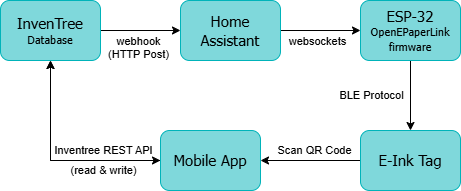
\includegraphics[width=0.9\textwidth]{arquitetura}
    \caption{Arquitetura geral}
    \label{fig:arquitetura}
\end{figure}

\subsubsection{Fluxo de atualização das etiquetas}

Sempre que o nome de uma gaveta é alterado no Inventree (quer manualmente quer utilizando a aplicação móvel), o plugin desenvolvido para o projeto deteta essa alteração e inicia automaticamente o processo de sincronização. O fluxo de atualização ocorre da seguinte forma:

\begin{enumerate}
    \item O utilizador altera o nome de uma localização no Inventree ou na aplicação;
    \item O plugin deteta a alteração;
    \item O plugin envia um pedido HTTP para o Home Assistant contendo a identificação da etiqueta e o novo conteudo a apresentar;
    \item O Home Assistant recebe o pedido e encaminha-o para o módulo OpenEPaperLink;
    \item O OpenEPaperLink comunica com o ponto de acesso ESP32;
    \item O ESP32 transmite a atualização para a etiqueta e-ink correspondente, que atualiza automaticamente a informação apresentada.
\end{enumerate}

Esta abordagem permite desacoplar o sistema de inventário do hardware responsável pelas etiquetas, tornando a solução mais moduklar e facilitando futuras evoluções.

\subsubsection{Tecnologias utilizadas}

A Tabela~\ref{tab:tecnologias} apresenta as principais tecnologias utilizadas durante o desenvolvimento do projeto.

\begin{table}[H]
    \centering
    \begin{tabular}{|1|p{10cm}|}
         \hline
         \textbf{Tecnologia} & \textbf{Finalidade} \\ \hline
         
         Inventree & 
         Sistema de gestão de inventário utilizado como fonte principal dos dados. \\ \hline

         Python &
         Desenvolvimento do plugin responsável pela sincronização dos dados. \\ \hline

         REST API &
         Comunicação entre os diferentes componentes do sistema. \\ \hline

         Home Assistant &
         Plataforma de automação utilizada como intermediário na atualização das etiquetas. \\ \hline

         OpenEPaperLink &
         Firmware responsável pela gestão do ponto de acesso e das etiquetas eletrónicas. \\ \hline

         ESP32 &
         Ponto de acesso responsável pela comunicação BLE com as etiquetas e-ink. \\ \hline

         React.js &
         Utilizado no desenvolvimento da aplicação móvel. \\ \hline

         Git e Github &
         Controlo de versões e sincronização entre os elementos da equipa. \\ \hline
         
    \end{tabular}
    \caption{Tecnologias utilizadas na solução desenvolvida.}
    \label{tab:tecnologias}
\end{table}

\subsubsection{Plugin do InvenTree}

O plugin foi desenvolvido em Python recorrendo ao sistema de extensões disponibilizado pelo InvenTree. A sua principal responsabilidade consiste em monitorizar alterações efetuadas às localizações do inventário e iniciar o processo de atualização das etiquetas.

Sempre que ocorre uma alteração ao nome de uma gaveta, o plugin constrói um pedido HTTP contendo a identificação necessária para identificar a etiqueta correspondente e o novo conteúdo e envia esse pedido para um endpoint previamente configurado no Home Assistant.

Esta solução permite que toda a lógica de comunicação com as etiquetas permaneça independente do sistema de inventário, reduzindo o acoplamente entre os diferentes componentes.

\subsubsection{Aplicação móvel}

Foi igualmente desenvolvida uma aplicação móvel que comunica diretamente com a REST API disponibilizada pelo InvenTree.

A aplicação permite consultar a informação do inventário, pesquisar componentes e visualizar o conteúdo das diferentes localizações. Adicionalmente, possibilita a atualização da informação armazenada no sistema, garantindo que todas as alterações são efetuadas diretamente na base de dados do inventário.

Entre as principais funcionalidades implementadas destacam-se:

\begin{itemize}
    \item consulta de componentes;
    \item pesquisa de localizações;
    \item localização de componentes;
    \item visualização do stock disponível;
    \item leitura de códigos QR para acesso rápido aos componentes de uma gaveta;
    \item atualização da informação através da API do Inventree.
\end{itemize}

\subsubsection{Dificuldades encontradas}

Durante o desenvolvimento do projeto foram identificados diversos desafios técnicos.

O principal desafio consistiu na integração entre diferentes plataformas, uma vez que cada sistema possui mecanismos próprios de comunicação e autenticação. Esta dificuldade foi ultrapassada através da utilização de REST APIs e da definição de um fluxo de comunicação bem estruturado. O Home Assistant também contribuiu para facilitar a integração dos diferentes componentes.

Outro desafio relacionou-se com a associação entre as localizações existentes no InvenTree e as respetivas etiquetas eletrónicas. Para esse efeito e com o objetivo de tornar a solução o mais adaptável possível foi colocado um identificador na descrição de cada localização que a liga à etiqueta correspondente.

Por último, foi necessário assegurar que a vida útil das etiquetas era suficiente para não serem necessárias substituições frequentes da bateria. Como tal adotamos medidas que permitem uma maior poupança de energia como atualizações menos frequentes mas suficientemente rápidas para se manterem utilizáveis. O firmware OpenEPaperLink foi essencial para este problema visto já ter sido desenvolvido tendo a eficiência energética em consideração.

\subsection{Solução desenvolvida}

Apresentar a solução desenvolvida na ótica do utilizador, com ajuda de screenshots.

\subsection{Validação}

Descrição da validação da solução desenvolvida (por exemplo, resultados de avaliação experimental, testes efetuados, feedback de utilizadores ou especialistas, etc.).


\section{Conclusões}


	
\subsection{Resultados alcançados} 	
 Sumariar os resultados alcançados e contribuições (em relação aos objetivos).
	
 No caso de trabalho em grupo, clarificar as contribuições individuais, em termos qualitativos e quantitativos (percentagem).
\subsection{Lições aprendidas} 	
 Refletir sobre as lições aprendidas (tendo em conta os objetivos de aprendizagem).
	
\subsection{Trabalho futuro} 
 
 Ideias de melhorias e trabalho futuro. 

\subsection{Impacto ODS}

Caso aplicável, identificar a contribuição do trabalho para os Objetivos de Desenvolvimento Sustentável (ODS) estabelecidos pelas
Nações Unidas (https://sdgs.un.org/goals), com vista a um futuro mais sustentável e inclusivo. 


\bibliographystyle{plain} 
\bibliography{refs} % Entries are in the refs.bib file
 
\end{document}
